\documentclass{knowdive}
\usepackage{color,soul}
\usepackage{subcaption}
\usepackage{fancyhdr}
\usepackage{lastpage}
\usepackage{textcomp}
\usepackage{lscape}
\usepackage{rotating}
\usepackage{multirow}
\usepackage{listings}
\usepackage[table,xcdraw]{xcolor}
\usepackage{amsmath}
\usepackage{graphicx}
\usepackage{enumerate}
\usepackage{hyperref}
\usepackage{rotating}
\graphicspath{ {images/} }

\usepackage{titlesec}
\titleformat{\section}{\LARGE\bfseries}{\thesection}{1em}{}

\usepackage{array, makecell}
%\hypersetup{
	%pdfauthor={Author1, \and Author2},
	%pdftitle={Collectives.State of the Art},
       %pdfkeywords = {},
      %pdfsubject={}
      %}
%\usepackage{hyperref}


\graphicspath{ {images/} }
\usepackage{comment}

\title{KGE 2022 - Project Report Template}

\author{Author1, ..., AuthorN}

\revisionhistory{
    \revision{0.1}{20.04.2020}{Fausto Giunchiglia}{Document created}
}
\newpage

\fancypagestyle{plain}{
  \fancyhf{}% Clear header/footer
  %\fancyhead[R]{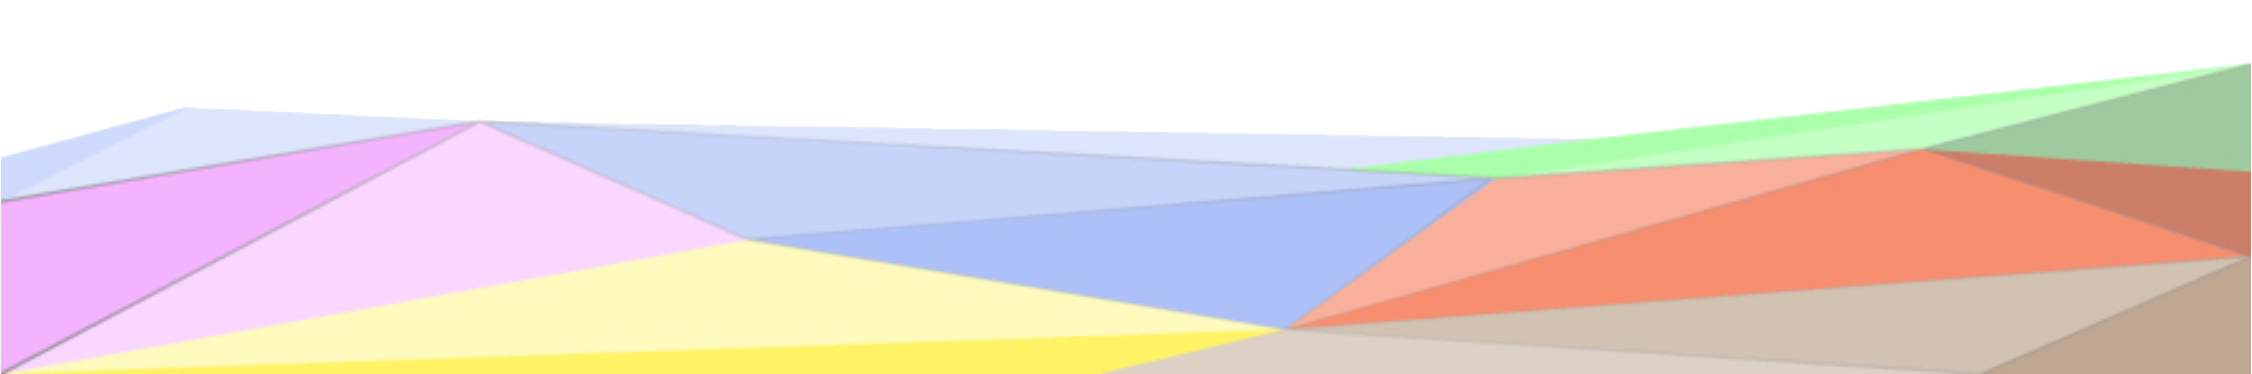
\includegraphics[width=1.0\linewidth,height=5pt]{Knowdive_color_bar}}% Right header
  \fancyfoot[L]{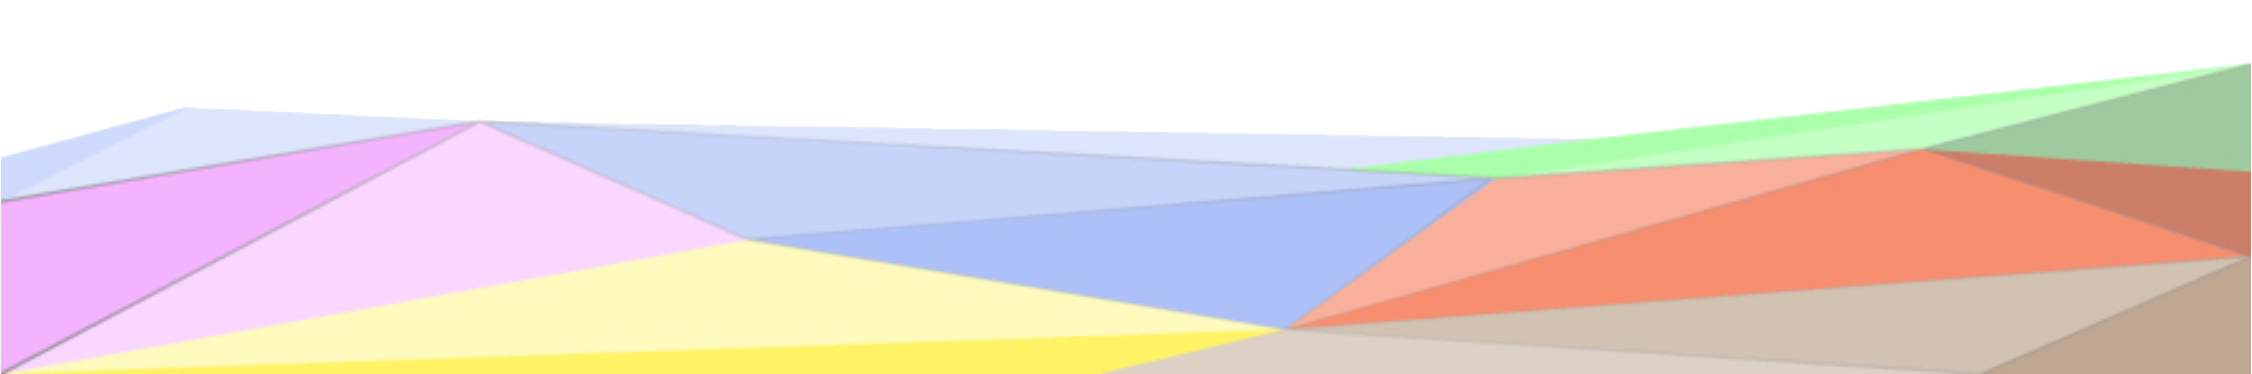
\includegraphics[width=1.0\linewidth,height=45pt]{Knowdive_color_bar}}% Left footer
  \fancyfoot[C]{Page \thepage\  / \pageref{LastPage}}
}

\pagestyle{plain}
%\makeglossaries
%input{glossaries}
\begin{document}
\maketitle
\begin{sloppypar}
\large
\begin{spacing}{1.05}
%\gls{latex}
%\gls{batex}
%\gls{eType}
%\printglossary

\section{Introduction}


Reusability is one of the main principles in the Knowledge Graph Engineering (KGE) process defined by iTelos. The KGE project documentation plays an important role in order to enhance the reusabiltiy of the resources handled and produced during the process. A clear description of the resources and the process developed, provides a clear understanding of the KGE project, thus serving such an information to external readers in order to exploit that in new projects.\\

The current document aims to provide a detailed report of the KGE project developed following the iTelos methodology. The report is structured, to describe:
\begin{itemize}
    \item Section 2: The project's purpose and the domain of interest and the resources involved (both schema and data resources) in the integration process.

    \item Section 2: The input resources considered by the KGE project. 
    
    \item Section 4, 5, 6, 7: The integration process along the different iTelos phases, respectively.
    
    \item Section 8: How the result of the KGE process (the KG) can be exploited.

    \item Section 9: Conclusions and open issues summary.
\end{itemize}
\section{Purpose and Domain of Interest (DoI)}


This section has to report and describe:
\begin{itemize}
    \item The project's purpose, by reporting the main Purpose as expressed by the final user.

    \item The definition of the project's Domain of Interest, by defining its boundaries in space and time.

\end{itemize}
\section{Data Sources}

This section has to report and describe the input resources considered:
\begin{itemize}  
    \item \textbf{Knowledge sources}: The sources for reference schemas and ontologies initially collected to satisfy the purpose along the KGE process. The knowledge resources initial metadata have to be reported here.
    
    \item \textbf{Data sources}: The sources for datasets initially collected to satisfy the purpose along the KGE process. The data resources initial metadata have to be reported here.
\end{itemize}

\section{Purpose Formalization}

The Purpose formalization section has to report:
        \begin{itemize}
            \item \textbf{Scenarios}: a set of usage scenarios, describing examples of usage of the Purpose.
            \item \textbf{Personas}: a set of real users examples acting  within the scenarios defined above. Each Persona is defined over a specific features included in the main Purpose.
            \item \textbf{Competency Questions (CQs)}: the list of CQs created considering the personas in the scenarios defined.
            \item \textbf{Entities identified}: the terms representing the entities to consider in the KGE project, classified using the popularity categories.
        \end{itemize}
\section{Inception}


This section aims to report the KGE sub process performed during the inception phase, by describing each activities both in schema and data layer.\\

\noindent Inception sub activities:
\begin{itemize}
    \item Resources collection/scraping
    \item Resources filtering and classification over common, core and contextual
    \item Resources knowledge definition/extraction
    \item Resources formatting (semi-formal transformation)
\end{itemize}

\noindent The report of the work done during the first phase of the methodology, has to includes also the description of the  different choices made, with their strong and weak points. In other words the report should provide to the reader, a clear description of the reasoning conducted by all the different team members. Moreover, the difficulties as well as open issues eventually involved in the inception phase sub process, should be reported.\\


\section{Informal Modeling}
This section is dedicated to the description of the informal modeling phase. Like in the previous section, it aims to describe the different sub activities performed by all the team members, as well as the phase outcomes produced.\\

\noindent More in details, this section provides a description of the following activities:
\begin{itemize}
    \item ER model description. Both the creation process (decisions taken) and the outcome have to be described.
    \item Teleology building.
    \item Datasets filtering and alignment with teleology.
    \item Phase open issues.
\end{itemize}

\noindent Like the previous phase, also the current one has to report the decision made during the phase activities, with the weak and strong point associate to them. If difficulties and/or open issue have been encountered, they should be reported as well.

\section{Formal Modeling}
This section is dedicate to the description of the formal modeling phase. Like in the previous section, the current one aims to describe the different sub activities performed by all the team members, as well as the phase outcomes produced.\\

\noindent More in details, this section provides a description of the following activities:
\begin{itemize}
    \item ETG generation
    \item Language alignment
    \item Formal data creation, by aligning datasets with the ETG created.
    \item Phase open issues
\end{itemize}

\noindent Like the previous phase, also the current one has to report the decision made during the phase activities, with the weak and strong point associate to them. If difficulties and/or open issue have been encountered, they should be reported as well.

\section{KGC}
This section is dedicate to the description of the KGC phase. Like in the previous section, the current one aims to describe the different sub activities performed by all the team members, as well as the phase outcomes produced.\\

\noindent More in details, this section provides a description of the following activities:
\begin{itemize}
    \item Data mapping. The mapping activities describe how the final KG is created. Provide a description of such activities for the datasets considered.  
    \item Entity matching (semantic heterogeneity). Describe how different representation of the same real world objects have been handled.
    \item Phase open issues
\end{itemize}


7
\section{Outcome Exploitation}

This section aims to provide a description of the KGE process outcome. Here you have to report the final Knowledge Graph information statistics (like, number of etypes and properties, number of entities for each etype, and so on). Moreover this section has to provide a description for the KG possible exploitation, like examples of queries executed, execution time, and so on.


\section{Conclusions \& Open Issues}
This section concludes the current document with final conclusions regarding the quality of the process and final outcome:
\begin{itemize}
    \item Did the project respect the scheduling expected in the beginning ?
    \item Are the final results able to satisfy the initial Purpose ?
        \begin{itemize}
            \item If no, or not entirely, why ? which parts of the Purpose have not been covered ?
        \end{itemize}
\end{itemize}


\noindent Moreover, this section aims to summarize the most relevant issues/problems remained open along the KGE process. The description of open issues has to provide a clear explanation about the problems, the approaches adopted while trying to solve them and, eventually, any proposed solution that has not been applied.

\end{spacing}
\end{sloppypar}
\end{document} 